
\zsavepos{header-1}

\zsavepos{header-1}\section{Experiments\zsavepos{header-2\zsavepos{header-2}}
\zsavepos{header-3}\zlabel{header}
}\zsavepos{header-3}\zlabel{header}

We conduct systematic experiments to answer \textit{Q1} and \textit{Q2} raised in Sec.~\ref{sec:intro}. We split the dataset into train, validation and test sets with 3:1:2 ratio. For \textit{Q1}, we collect state-of-the-art baselines and evaluate them in \benchmark. We further introduce three metrics based on the underlying structure of graphs and the surface form of elements. Specifically, we use the BLEU scores to measure the performance of actor, action and constraint extraction and F1 scores to measure the performance of gateway prediction. Besides, the performance of flow prediction is measured via soft F1 scores~\cite{tandon-etal-2020-dataset}, which is computed based on the BLEU scores of associated textual elements. For \textit{Q2}, we involve Flan-T5~\cite{chung2022scaling}, ChatGPT~\cite{ouyang2022training} and Llama2~\cite{touvron2023llama} in \benchmark to show their potentials and improve their performance using a self-refine strategy.

\zsavepos{header-1}

\zsavepos{header-1}\subsection{Performance of Baselines~(\textit{Q1\zsavepos{header-2\zsavepos{header-2}}
\zsavepos{header-3}\zlabel{header}
}
\zsavepos{header-3}\zlabel{header}
)}

\zsavepos{header-1}\paragraph{Baselines\zsavepos{header-2}}\zsavepos{header-3}\zlabel{header}

We collect five baselines:
\begin{itemize}
    \item  \citet{sonbol2023machine} uses rules to extract sequential, exclusive, and parallel actions with a few data constraints.
    \item \citet{neuberger2023beyond} designs a pipeline to extract sequential actions and organize partial non-sequential actions, ignoring all constraints and inclusive gateways.
    \item \citet{sholiq2022generating} extracts actions, exclusive gateways, and parallel gateways based on a pre-defined representation of the procedural graph.
    \item  PET~\cite{bellan2023pet} trains a sequence tagging model to extract actions with a few constraints and uses rules to construct the final graph.
   \item  CIS~\cite{bellan2022leveraging} presents a rough attempt to use LLMs\footnote{The LLM used in \citet{bellan2022leveraging} is GPT3. We replace it with ChatGPT in the current setting for a fair comparison.} for action extraction via few-shot in-context learning and constructs the graphs via  handwritten rules.
\end{itemize}

\zsavepos{header-1}\paragraph{Results\zsavepos{header-2}}\zsavepos{header-3}\zlabel{header}

As shown in Table~\ref{exp_results}~(Rows 1-5), existing studies are far from solving this task well, especially when organizing the logical structure of graphs~(cf., the results on gateways and flows). This is because either rules or neural models are derived from limited data, leading to an incomplete coverage of all elements and an incomprehensive understanding of complex documents. Additionally, we have the following observations: \par
%
1) Heuristic methods~(Row 1-3) perform poorly for actor, action and constraint extraction. The reason is that hand-written rules fail to understand various expressions and coreferences, resulting in poor generalization. \par
2) PET~(Row 4), though being a customized deep neural model, only performs slightly better than heuristic methods. This is because the PET model is only trained on 45 samples and utilizes several rules to construct the flows. \par
3)  We conjecture the reason why all baselines only meet part of the requirements of optimal procedural graphs lies in the huge cost of writing rules and annotating data. We believe this issue can be alleviated with the dataset created in Sec.~\ref{sec:data}.\par
4)  It is not surprising that CIS~(Row 5) achieves the highest scores on the action and actor extraction among these baselines, as it gains more power to understand word meanings from the LLM. Note that, the increase in flow prediction between PET and CIS also comes from more accurate action extraction instead of more delicate rules to construct the graph. This increase further encourages us to investigate more potentials of LLMs in procedural graph extraction. \par
5)  All baselines perform poorly on flow prediction, indicating the challenge of understanding logical structures in documents. This motivates us to find out, besides an in-depth study of LLMs, what else matters to construct the logic in graphs.
%
\zsavepos{header-1}

\zsavepos{header-1}\subsection{Performance of LLMs~(\textit{Q2\zsavepos{header-2\zsavepos{header-2}}
\zsavepos{header-3}\zlabel{header}
}
\zsavepos{header-3}\zlabel{header}
)}

\zsavepos{header-1}\paragraph{LLMs\zsavepos{header-2}}\zsavepos{header-3}\zlabel{header}

We investigate three advanced LLMs. The first one is ChatGPT~\cite{ouyang2022training}, which is good at information comprehension and text generation. Different from CIS~\cite{bellan2022leveraging}, we use our high-quality dataset to apply few-shot in-context learning~(ICL) on ChatGPT. The other two~(Flan-T5~\cite{chung2022scaling} and Llama2~\cite{touvron2023llama}) are open-source alternatives to ChatGPT. Besides ICL, we also deploy the alternatives with supervised fine-tuning strategies.

\zsavepos{header-1}\paragraph{Results\zsavepos{header-2}}\zsavepos{header-3}\zlabel{header}

As expected, the LLMs~(Rows 6-10) update state-of-the-art results on all metrics, especially for actor, action and constraint extraction. However, for gateway and flow predictions, all LLMs can hardly get $>0.5$ F1 scores, exhibiting their weakness in arranging logical structures of graphs. We also have the following observations: \par
1) Our high-quality dataset significantly promotes LLMs' ability on procedural graph extraction. A piece of direct evidence is that we see a rising trend between the results on Rows 5 and 8, whose only difference lies in the data used in the few-shot ICL. Another piece of evidence is that the gap between Flan-T5 and Llama2 is rapidly narrowed after using more data from our dataset for tuning. \par
2) The procedural knowledge, especially the logical structure of non-sequential actions, has been overlooked during the initial training of LLMs. This is demonstrated by the fact that fine-tuned LLMs perform better than few-shot LLMs. The Llama2 model even beats ChatGPT after learning more procedural knowledge from supervised fine-tuning. \par
3) LLMs, including CIS, show significant potential for actor, action and constraint extraction, indicated by the large improvements compared with Rows 1-4. This is because LLMs are good at understanding lengthy contexts and thus have the advantage of identifying meaningful elements from procedural documents. We also believe that the emergence of more powerful LLMs in the future will continue to promote better results on these metrics. \par
4) We believe the biggest challenge for LLMs to extract accurate procedural graphs lies in the lack of logic reasoning ability among actions, especially non-sequentially executed ones. The supporting evidence is that, though largely surpassing baselines on the actor, action and constraint extractions, LLMs don't present such impressive improvements in gateway extraction. This implies that we can boost LLMs' performances by paying extra attention to non-sequential logic prediction.

\begin{figure}[!t]
    \zsavepos{figure-1}
    \zsavepos{figure-1}
    \centering
    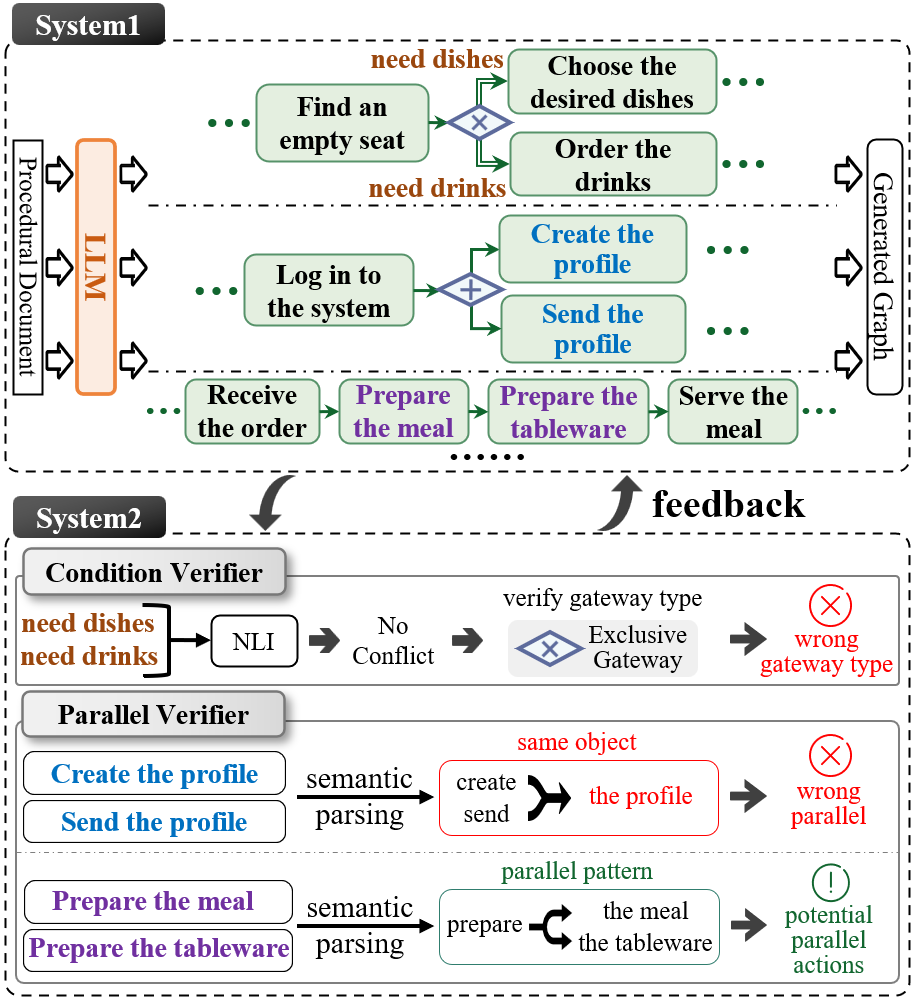
\includegraphics[width=1\linewidth]{figures/Method.png}
    \zsavepos{figure-2}

    \zsavepos{figure-2}
    \zsavepos{figurecap-1}
    \zsavepos{figurecap-1}\caption{The self-refine strategy, in which ``System1'' extracts procedural graphs and ``System2'' verifies gateways of graphs and provides feedback for refinement.
    }\zsavepos{figurecap-2}\zsavepos{figurecap-2}
    \label{fig:method}
    \zlabel{figure}

    \zlabel{figure}
\end{figure}

\phantom{Invisible Text}
\vspace{-\baselineskip}

\zsavepos{header-1}

\zsavepos{header-1}\subsection{Self-refine Strategy\zsavepos{header-2\zsavepos{header-2}}
\zsavepos{header-3}\zlabel{header}
}\zsavepos{header-3}\zlabel{header}

To overcome the above-mentioned challenge, inspired by \citet{nye2021improving, madaan2023self}, we design a self-refine strategy to help LLMs gain logic reasoning ability among actions from iterative feedback and refinement. As shown in Figure~\ref{fig:method}, it consists of two systems --- ``System1'' is used to directly extract procedural graphs from documents, ``System2'' is used to verify the extracted graphs and provide feedback for further refinement of ``System1''. In ``System2'', we center on the shortest slab and carefully examine the gateway prediction results using the condition and parallel verifiers.

\zsavepos{header-1}\paragraph{Condition Verifier\zsavepos{header-2}}
\zsavepos{header-3}\zlabel{header}
 We design the condition verifier to handle both exclusive and inclusive gateways, whose key difference lies in the conditions followed by gateways. It is worth noticing that, with the exclusive gateway, there is always one and only one condition that can be met. Accordingly, we suppose if the conditions hold conflict, the gateway should be the exclusive one; otherwise, it should be the inclusive one. Particularly, we use a pre-trained natural language inference~(NLI) model~\cite{liu2019roberta} to detect the conflict and verify gateways. For example, after feeding ``need dishes'' and ``need drinks'' into the NLI model, we get ``No Conflict''. This suggests the gateway should be the inclusive one, which is different from the result predicted by ``System1''. In this case, the condition verifier is triggered to provide feedback to refine ``System1''.
%
\zsavepos{header-1}\paragraph{Parallel Verifier\zsavepos{header-2}}
\zsavepos{header-3}\zlabel{header}
 We further design the parallel verifier to reorganize the actions performed in parallel. We notice that if the actions act on the same object, they can never be executed in parallel. Given that, we extract the objects of actions using the semantic parsing tool and determine the parallel gateway based on these objects. For example, as ``create the profile'' and ``send the profile'' have the same object ``the profile'', they cannot be performed in parallel. Besides, the optimal procedural graph is expected to help users in a time-saving way~\cite{miller1979humanistic}. Thus, we further prepare another type of feedback by examining the sequential actions. For example, as ``prepare the meal'' and ``prepare the tableware'' have different objects, they have a big chance to be performed in parallel. We provide ``System1'' with both types of feedback for the refinement of mistakes on parallel gateways.
%
\begin{figure}[t]
    \zsavepos{figure-1}
    \zsavepos{figure-1}
    \centering
    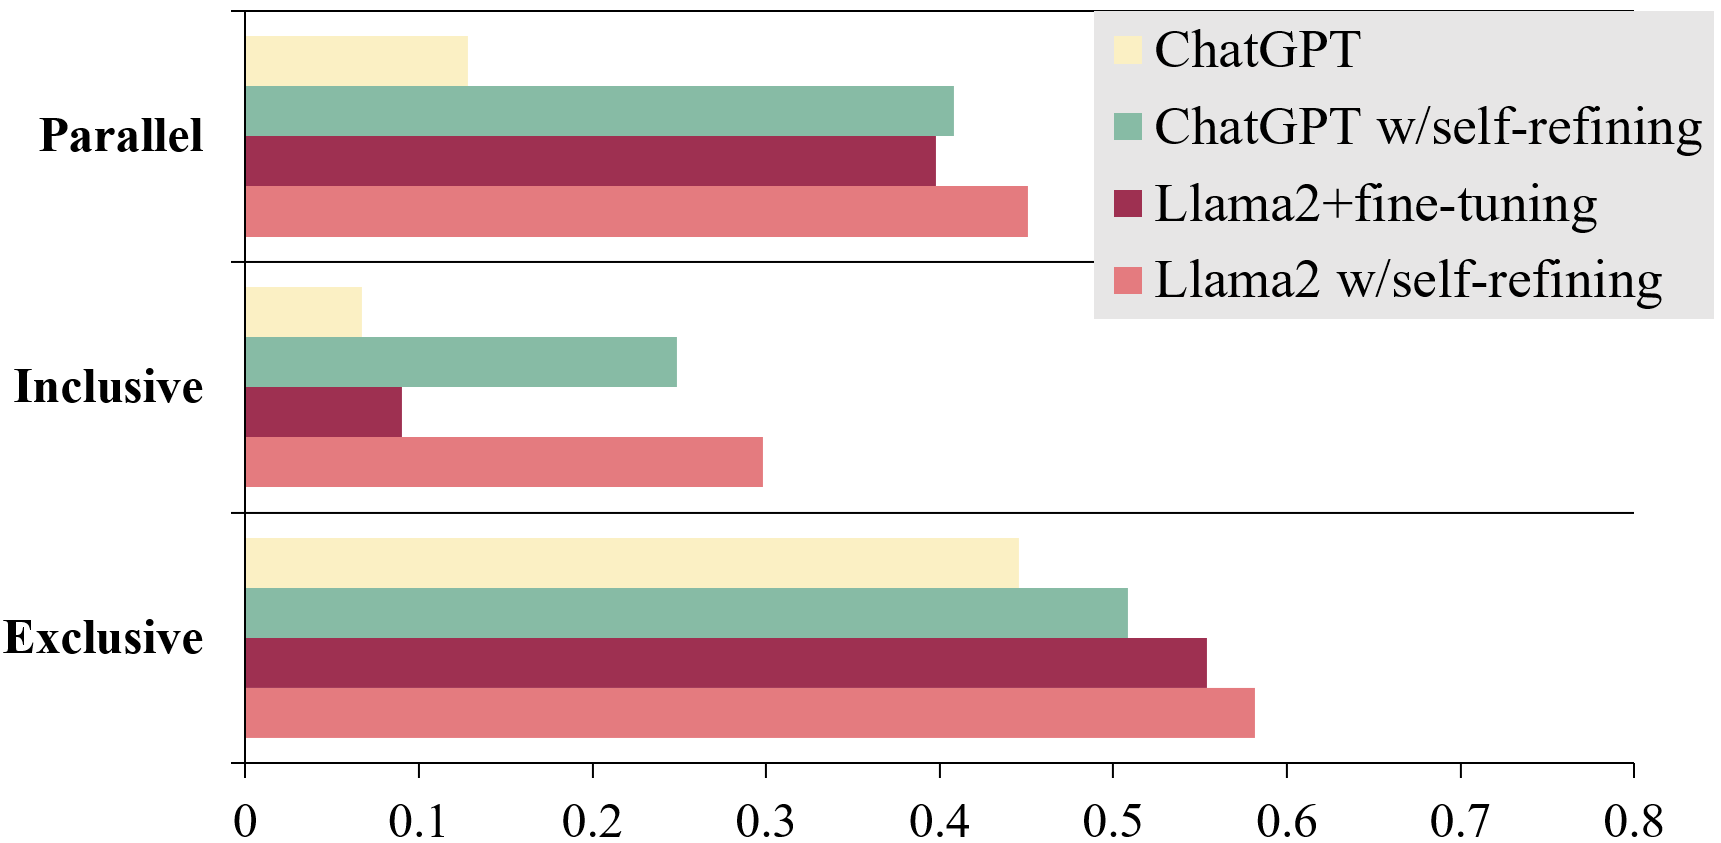
\includegraphics[height=3.6cm]{figures/improve.png}
    \zsavepos{figure-2}

    \zsavepos{figure-2}
    \zsavepos{figurecap-1}
    \zsavepos{figurecap-1}\caption{F1 scores on gateway predictions of LLMs and their variants with our self-refine strategy.
    }\zsavepos{figurecap-2}\zsavepos{figurecap-2}
    \label{fig:improve}
    \zlabel{figure}

    \zlabel{figure}
\end{figure}

\phantom{Invisible Text}
\vspace{-\baselineskip}

\zsavepos{header-1}\paragraph{Results\zsavepos{header-2}}\zsavepos{header-3}\zlabel{header}

We apply the self-refine strategy to the top-two winners in Table~\ref{exp_results}, i.e., ChatGPT and fine-tuned Llama2. As shown in Figure~\ref{fig:improve}, both ChatGPT and fine-tuned Llama2 have better performances with the help of our self-refine strategy. More surprisingly, there are significant improvements in inclusive gateway extraction, whose previous scores are extremely poor. This indicates that, with effective strategies, LLMs have the potential to gain logic reasoning ability among actions including non-sequential ones. The improvement of Llama2 is not as large as that of ChatGPT. This is because the model's gain from the self-refine strategy drops as it encounters more procedural knowledge. This suggests the importance of incorporating the learning of procedural knowledge during the pre-training stage of LLMs, which will be beneficial for LLMs' logic reasoning ability.

\begin{figure}[t]
    \zsavepos{figure-1}
    \zsavepos{figure-1}
    \centering
    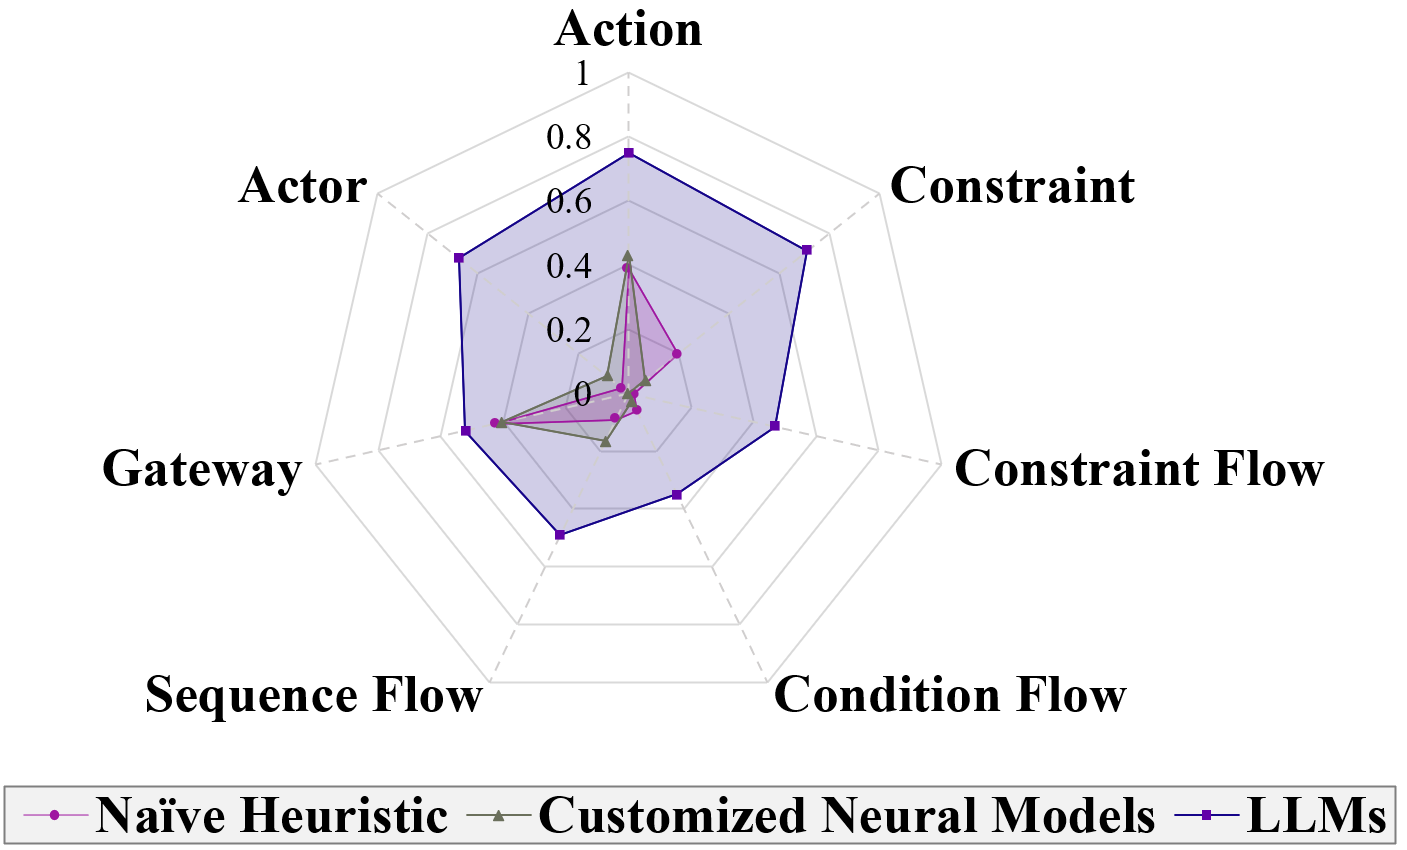
\includegraphics[height=4cm]{figures/Radar.png}
    \zsavepos{figure-2}

    \zsavepos{figure-2}
    \zsavepos{figurecap-1}
    \zsavepos{figurecap-1}\caption{Best performances of heuristics, customized neural models and LLMs on seven dimensions.
    }\zsavepos{figurecap-2}\zsavepos{figurecap-2}
    \label{fig:Radar}
    \zlabel{figure}

    \zlabel{figure}
\end{figure}

\phantom{Invisible Text}
\vspace{-\baselineskip}

\zsavepos{header-1}\paragraph{Auxiliary Analysis\zsavepos{header-2}}\zsavepos{header-3}\zlabel{header}

We group the methods into three sets, i.e., the na\"ive heuristics~(rows 1-3), customized neural models~(row 4), and LLMs~(rows 5-10). Towards a clear understanding of the advantages and challenges, we report the best performances of each type of method on seven dimensions in Figure~\ref{fig:Radar}. Even with the highest scores, heuristic methods and customized neural models exhibit poor performance across all dimensions and can hardly handle condition and constraint flows due to their neglect of the logical structure in documents. LLMs show substantial improvements compared to the others in all dimensions except for the gateway. This suggests that even the powerful LLMs face challenges in managing non-sequential actions, which is also the main challenge when conducting optimal procedural graph extraction.
%